\chapter{Goniometrie}
\label{chap:goniometrie}

Regelmatig voeren we berekeningen uit waarin \'e\'en of meerdere hoeken 
voorkomen: de hoogte van een gebouw die je niet kunt opmeten, de 
koers van een schip, de kracht op een schuin vlak, of de lengte van een 
dwarsligger in een constructie. 

Zodra in zo'n situatie een \emph{rechthoekige} driehoek te herkennen is, biedt de goniometrie (letterlijk ``hoekmeting'', van het Griekse \textit{g\`onia}, hoek, en \textit{metron}, maat) de gereedschappen om de ontbrekende hoeken en zijdes te berekenen.

    \begin{figure}[H]
        \centering
        \begin{tikzpicture}
          \driehoek{$C$}{$A$}{$B$}{$b$}{$c$}{$a$}{$\alpha$}{$\beta$}  
        \end{tikzpicture}
        \caption{Een rechthoekige driehoek}
        \label{fig:rechthoekigedriehoek}
    \end{figure}

De kern van de goniometrie is opvallend simpel: in rechthoekige 
driehoeken met dezelfde scherpe hoek $\alpha$ zijn de 
\emph{verhoudingen} tussen de zijdes altijd gelijk, hoe groot of klein 
de driehoek ook is. Dat betekent dat elke verhouding alleen van de 
hoek afhangt. 

In dit hoofdstuk leren we deze verhoudingen toepassen: zijdes en 
hoeken in rechthoekige driehoeken berekenen, hoeken omrekenen van 
graden naar radialen, en de goniometrische verhoudingen gebruiken in 
niet-rechthoekige driehoeken (met de sinus- en cosinusregel).

\textbf{Let op:} controleer v\'o\'or elke berekening of je rekenmachine 
in de juiste modus staat (DEG voor graden, RAD voor radialen). Een 
verkeerde modus is de veelgemaakte fout.

% Regelmatig voeren we berekeningen uit, waarin \'e\'en of meerdere hoeken voorkomen. Voor een scherpe hoek $\alpha$ kunnen we 3 goniometrische verhoudingen defini\"eren. Deze laten zich het gemakkelijkst aflezen in de rechthoekige driehoek $ABC$ (de hoek bij $C$ is recht):


\vspace{-0.5cm}
\section{SOSCASTOA en Pythagoras}
Voor de bovenstaande rechthoekige driehoek kunnen we 3 goniometrische verhoudingen defini\"eren om berekeningen uit te voeren. Deze kunnen we onthouden met het ezelsbruggetje SOSCASTOA: 
\regel{}{\sin \alpha=\frac{\text{overstaande zijde}}{\text{schuine zijde}}}
\regel{}{\cos \alpha=\frac{\text{aanliggende zijde}}{\text{schuine zijde}}}
\regel{}{\tan \alpha=\frac{\text{overstaande zijde}}{\text{aanliggende zijde}}}

% Deze regels toegepast op de driehoek hierboven, geeft ons: 
% \[
%     \sin \alpha = \frac{a}{c} \qquad \cos \alpha = \frac{b}{c} \qquad \tan \alpha = \frac{a}{b}
% \]
% 
Om deze regels te kunnen toepassen, is het dus belangrijk om te weten wat de overstaande, aanliggende en schuine zijde van de driehoek zijn. De schuine zijde spreekt voor zich. Maar voor de andere twee licht het er maar net aan vanuit welke hoek je kijkt. Zie hiervoor het onderstaande plaatje, hierin is in rood aangegeven hoe de zijdes heten gezien vanuit hoek $\alpha$ en in het blauw vanuit hoek $\beta$.
{
\shorthandoff{"}
\begin{center}
\begin{tikzpicture}[scale=1.2]
    % Define 3 coordinates:
    \coordinate [label=left:$C$]  (A) at (1cm,-2cm);
    \coordinate [label=right:$A$] (B) at (6cm,-2cm);
    \coordinate [label=above:$B$] (C) at (1cm,1cm);
    
    % Draw traingle:
    \draw (A) -- node[align=center] { \\ \\ \\ 
            \small \color{red}  Aanliggende zijde \\ 
            \small \color{blue} Overstsaande zijde}
        (B) -- 
        (C) -- node[align=center, sloped] { \\ \\ \\ 
            \small \color{blue} Aanliggende zijde \\ 
            \small \color{red}  Overstsaande zijde}
        cycle;
    
    % Radius of angles:
    %\draw pic[draw,angle radius=1cm,"$\alpha$"] {angle=B--A--C};
    \draw (1cm,-2cm) rectangle (1.4cm,-1.6cm);
    \draw pic[draw,angle radius=1cm,"\color{red}$\alpha$"  shift={(-8mm,2mm)}] {angle=C--B--A};
    \draw pic[draw,angle radius=1cm,"\color{blue}$\beta$" shift={(3mm,-7mm)}]  {angle=A--C--B};
\end{tikzpicture}
\end{center}
}
Daarnaast geldt voor de zijdes van alle rechthoekige driehoeken de stelling van Pythagoras:
\regel{}{a^2+b^2=c^2}
Tenslotte is het goed om te weten dat de som van alle hoeken voor iedere rechthoekige driehoek $180^{\circ}$ is.

Voorbeelden:
\begin{enumerate}
    \item Bepaal in onderstaande figuur de lengte van de schuine zijde $c$. Bepaal daarna voor hoek $\alpha$ de sinus, de cosinus en de tangens. \\

    Oplossing: Pythagoras: 
    \begin{align*}
        3^2+4^2&=c^2 \\
        9+16&=c^2 \\
        25&=c^2 \\
        c&=\sqrt{25} = 5
    \end{align*}
    \[
        \sin \alpha = \frac{3}{5} \qquad \cos \alpha = \frac{4}{5} \qquad \tan \alpha = \frac{3}{4}
    \]

    \item Bepaal in onderstaande figuur de lengte van de rechthoekszijde $b$. Bepaal daarna voor hoek $\beta$ de sinus, de cosinus en de tangens
\end{enumerate}


\section{Hoeken berekenen met een rekenmachine}
Een hoek drukken we meestal uit in graden. Zo komt een rechte hoek overeen met $90^{\circ}$. Als de grootte van een hoek bekend is, dan kan de sinuswaarde, de cosinuswaarden en de tangenswaarde van die hoek met de rekenmachine worden bepaald.

Voorbeelden
\begin{enumerate}
    \itemsep1em
    \item Ga uit van een hoek $\alpha$ van $40^{\circ}$, dus: $\alpha=40^{\circ}$
          Dan kunnen we met de rekenmachine berekenen: 
          \begin{align*}
            \sin\alpha &=\sin 40^{\circ} \approx 0.643 \\
            \cos\alpha &=\cos⁡ 40^{\circ} \approx 0.766 \\
            \tan\alpha &=\tan⁡ 40^{\circ} \approx 0.834
          \end{align*}
          
    \item Ga uit van een hoek $\beta$ van $55^{\circ}$. \\
          Bereken: $\sin⁡\beta$, $\cos\beta⁡$ en $\tan\beta $
          
    \item In onderstaande rechthoekige driehoek is zijde $a=4$ en hoek $\alpha=35^{\circ}$. \\
          \begin{center}
              \begin{tikzpicture}
                \driehoek{$C$}{$A$}{$B$}{$b$}{$c$}{$a=4$}{$35^{\circ}$}{$\beta$}
              \end{tikzpicture}
          \end{center}
          Bereken de zijden $b$ en $c$. Bereken ook de hoek $\beta$. \\

          Oplossing:
          \begin{align*}
          \tan 35^\circ &= \frac{4}{b} \implies b = \frac{4}{\tan 35^\circ} \approx \frac{4}{0.7002} \approx 5.713 \\[0.5em]
          \sin 35^\circ &= \frac{4}{c} \implies c = \frac{4}{\sin 35^\circ} \approx \frac{4}{0.5736} \approx 6.974 \\[0.5em]
          \beta &= 180^\circ - 90^\circ - 35^\circ = 55^\circ
          \end{align*}

    \item In onderstaande rechthoekige driehoek is zijde $a = 8$ en hoek $\beta = 25^{\circ}$. \\
          \begin{center}
              \begin{tikzpicture}
                \driehoek{$C$}{$A$}{$B$}{$b$}{$c$}{$a=8$}{$25^{\circ}$}{$\beta$}
              \end{tikzpicture}
          \end{center}
          Bereken de zijden $b$ en $c$. Bereken ook de hoek $α$.

    \item Een balk is onder een bepaalde hoek $\gamma$ ingeklemd in de grond. Aan het         uiteinde van de balk hangt een gewicht, welke met een verticale kracht $F$          van 250 newton aan die balk trekt (zie onderstaande figuur). Deze kracht $F$        maakt een hoek van $50^\circ$ met de balk.\\

    \begin{center}
        % \begin{tikzpicture}
        %   \def\gamma{55}
        %   \def\Lrod{4}
        %   \def\dOver{0.7}
        %   \def\ang{50}
        %   \def\FYlen{2}
        %   \def\Flen{2.6}
        
        %   \coordinate (O) at (0,0);
        %   \coordinate (T) at ({\Lrod*cos(\gamma)},{\Lrod*sin(\gamma)});
        %   \coordinate (A) at ({(\Lrod+\dOver)*cos(\gamma)},{(\Lrod+\dOver)*sin(\gamma)});
        %   \coordinate (FY) at ($(A)+({\FYlen*cos(\gamma+180+\ang)},{\FYlen*sin(\gamma+180+\ang)})$);
        %   \coordinate (F) at ($(A)+(0,-\Flen)$);
        
        %   % GROUND
        %   \draw[thick] (-0.5,0) -- (6,0);
        %   \draw[thick, dashed] (0.9,0) arc (0:\gamma:0.9);
        %   \node at ({\gamma/2}:1.3) {$\gamma$};
        
        %   % ROD (incline)
        %   \draw[very thick, brown!60!black, double] (O) -- (T);
        
        %   % PARALLELOGRAM CONSTRUCTION (dashed)
        %   \draw[green!50!black, dashed] (T) -- (F);
        %   \draw[green!50!black, dashed] (FY) -- (F);
        
        %   % FORCE VECTORS
        %   \draw[->, green!50!black, thick] (A) -- (T) node[midway, above left] {$F_x$};
        %   \draw[->, green!50!black, thick] (A) -- (FY) node[right] {$F_y$};
        %   \draw[->, green!50!black, thick] (A) -- (F) node[below] {$F$};
        
        %   % ANGLE ARC BETWEEN F_x AND F_y
        %   \draw[dashed] ($(A)+({0.8*cos(\gamma+180)},{0.8*sin(\gamma+180)})$) arc (\gamma+180:\gamma+180+\ang:0.8);
        %   \node at ($(A)+({1.1*cos(\gamma+180+\ang/2)},{1.1*sin(\gamma+180+\ang/2)})$) {$50^{\circ}$};
        % \end{tikzpicture}
        
        \begin{tikzpicture}[
          >=Stealth,
          every node/.style={font=\small},
          vec/.style={-{Stealth[length=2.5mm]}, mygreen, thick},
          dvec/.style={mygreen, thick, dashed}
        ]
        
          % ground line
          \coordinate (P0) at (0,0);
          \coordinate (Gr) at (2,0);
          \draw[thick] (-0.6,0) -- (7,0);
        
          % incline (double rail line), top point T
          \coordinate (T) at ($(P0)+(40:5.5)$);
          \draw[very thick, double distance=5pt, line cap=round]
            (P0) -- (T);
        
          % force vector tips
          \coordinate (A) at ($(T)+(220:2.1)$); % F_x tip
          \coordinate (B) at ($(T)+(270:3)$);   % F tip
          \coordinate (C) at ($(T)+(B)-(A)$);   % F_y tip (parallelogram rule)
        
          % dashed completion lines
          \draw[dvec] (A) -- (B);
          \draw[dvec] (B) -- (C);
        
          % force vectors from T
          \draw[vec] (T) -- (A) node[above left, black] {$F_x$};
          \draw[vec] (T) -- (B) node[below, black] {$F$};
          \draw[vec] (T) -- (C) node[right, black] {$F_y$};
        
          % angle gamma at foot of incline
          % \draw pic[draw=blue, angle radius=9mm, angle eccentricity=1.5,
                    % "$\gamma$"] {angle=Gr--P0--T};

          % 50 degree angle at T  
          \draw[thick, dashed] ($(T)+(226:0.9)$) arc (220:270:0.9);
          \node at ($(P0)+(32:4.4)$) {$50^\circ$};
        
          % 50 degree angle at T
          \draw[thick, dashed] (1,0) arc (0:35:1);   
          \node at (20:1.4) {$\gamma$};
        
        \end{tikzpicture}
        \end{center}
    
          De kracht $F$ kunnen we ontbinden in 2 componenten: een kracht $F_x$, welke langs de balk valt, en een kracht $F_y$, welke loodrecht op de balk staat. \\
            
          Bereken de grootte van deze componenten. Bereken ook de grootte van de hoek $\gamma$

          Oplossing: 
            \begin{align*}
            \cos 50^\circ &= \frac{F_x}{F} \implies F_x = F \cdot \cos 50^\circ = 250 \cdot \cos 50^\circ \approx 160.7 \text{ newton} \\[0.5em]
            \sin 50^\circ &= \frac{F_y}{F} \implies F_y = F \cdot \sin 50^\circ = 250 \cdot \sin 50^\circ \approx 191.5 \text{ newton} \\[0.5em]
            \gamma &= 180^\circ - 90^\circ - 50^\circ = 40^\circ
            \end{align*}
    \item Een voorwerp wordt met een snelheid $V$ van 12 $m/s$ weggeschoten onder een hoek van $65^{\circ}$ (zie onderstaande figuur). \\

    \begin{center}
    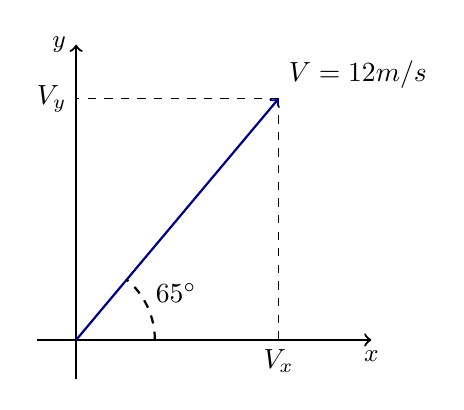
\begin{tikzpicture}[scale=1]%,cap=round,>=latex]
      \def\R{4}
      \def\ang{50}
      \coordinate (O) at (0,0);
      \coordinate (X) at (3.75,0);
      \coordinate (Y) at (0,3.75);
      \coordinate (R) at (\ang:\R);
      \coordinate (Rx) at ({\R*cos(\ang)},0);
      \coordinate (Ry) at (0, {\R*sin(\ang)});
      
      % AXIS
      \draw[->,thick] (-0.5,0) -- (X) node[below] {\small $x$};
      \draw[->,thick] (0,-0.5) -- (Y) node[left] {\small $y$};
      
      % PHASOR
      \draw[dashed] (R) -- (Rx) node[below]{$V_x$};;
      \draw[dashed] (R) -- (Ry) node[left]{$V_y$};
      \draw[->, blue!50!black, thick] (O) -- (R) node[above right] {\color{black}$V=12m/s$};
      \draw[thick, dashed] (1,0) arc (0:\ang:1);   
      \node at ({\ang/2}:1.4) {$65^{\circ}$};
    \end{tikzpicture}
    \end{center}
    
    Deze snelheid kunnen we ontbinden in 2 componenten: Een horizontale snelheid $V_x$ en een verticale snelheid $V_y$. \\
    
    Bereken de grootte van deze componenten \\ 

    We beschouwen de uitdrukking $y=\sin⁡20^\circ$. We kunnen de waarde van y berekenen met de rekenmachine m.b.v. de $\sin$-knop (rekenmachine instellen op graden!): $y=0,34202$. \\
    
    Bij deze vraag is de hoek bekend, en moet de onbekende sinuswaarde worden berekend. \\
    
    Beschouw nu de uitdrukking $\sin\alpha=0.62518$.
    We kunnen de waarde van de hoek $\alpha$ berekenen met de rekenmachine m.b.v. de $\sin^{-1}$-knop.\\
    
    Als we de rekenmachine instellen op graden, dan vinden we de hoek $\alpha=38.7^\circ$.\\
    
    Bij deze vraag is de sinuswaarde bekend, en moet de onbekende hoek worden berekend.
    Deze laatste vraag is het omgekeerde probleem (of inverse probleem) van de eerste vraag. \\
    
    Het bepalen van de onbekende hoek $\alpha$ uit de vergelijking $\sin\alpha=0.62518$ gebeurt dus met de $\sin^{-1}$-knop van de rekenmachine. \\
    
    Als je dit wilt opschrijven, dan kun je dit als volgt noteren:
    \begin{align*}
        \sin\alpha&=0.62518 \\
        \alpha&=\sin^{-1}⁡0.62518 \\
        \alpha&\approx38.7^\circ
    \end{align*}

    \item In onderstaande rechthoekige driehoek is zijde $a=3$ en zijde $c=7$. \\
          \begin{center}
              \begin{tikzpicture}
                \driehoek{$C$}{$A$}{$B$}{$b$}{$c=7$}{$a=3$}{$\alpha$}{$\beta$}        
              \end{tikzpicture}
          \end{center}
    
          Bereken de hoek $\alpha$ en de zijde $b$

        \begin{align*}
        \sin \alpha &= \frac{a}{c} = \frac{3}{7} \\
        \alpha &= \sin^{-1}\!\left(\frac{3}{7}\right) \approx 25.4^\circ \\[0.5em]
        \cos \alpha &= \frac{b}{c} \\
        \cos 25.4^\circ &= \frac{b}{7} \\
        \implies b &= 7 \cdot \cos 25.4^\circ \\
        b&\approx 6.32
        \end{align*}

    \item In onderstaande rechthoekige driehoek is zijde $a=4$ en zijde $c=11$. \\
          \begin{center}
              \begin{tikzpicture}
                \driehoek{$C$}{$A$}{$B$}{$b$}{$c=11$}{$a=4$}{$\alpha$}{$\beta$}        
              \end{tikzpicture}
          \end{center}
          Bereken de hoek $\beta$ en de zijde $b$
\end{enumerate}

\section{Graden en radialen}
Een hoek kun je aangeven in graden, bijvoorbeeld $\alpha=35^\circ$. De eenheid graden behoort niet tot het SI-stelsel. Een andere eenheid voor de hoek is de radiaal, afgekort met rad. Bijvoorbeeld $\beta=0,48$ rad. Deze eenheid behoort wel tot het SI-stelsel. 
\begin{center}
    \begin{figure}[H]
        \centering
        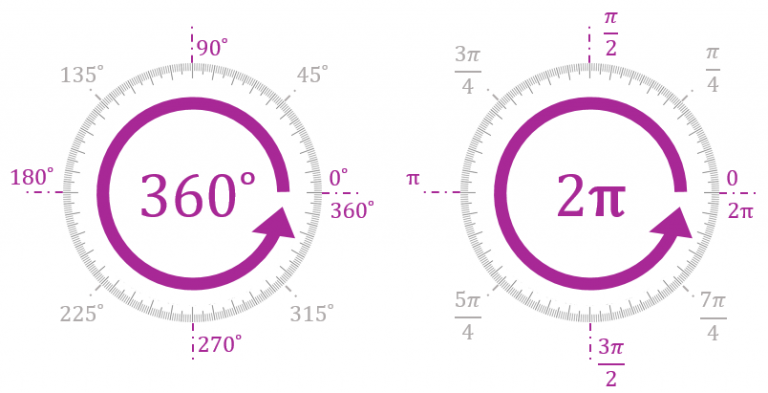
\includegraphics[width=0.8\linewidth]{pictures/figuren/rad_deg.png}
        \caption{Een cirkel onderverdeeld in $360^\circ$ graden en $2\pi$ radialen}
        \label{fig:rad_deg}
    \end{figure}
\end{center}
\vspace{-0.8cm}
Het verband tussen graden en radialen: Bij een volledige rondgang langs een cirkel behoort een draaiingshoek van $360^\circ$ of $2\pi$ radialen.

Zodat: 
\begin{align*}    
    2\pi \text{ radialen} &= 360^\circ \\
    1 \text{ radiaal} & = \frac{360}{2\pi}^\circ 
\end{align*}
Dus:
\regel{}{1\text{ radiaal} = \frac{180}{\pi}^\circ}

Hieruit kunnen we berekenen, dat: $1 \text{ radiaal} \approx 57.3^\circ$. Evenzo kunnen we concluderen:

\regel{}{1^\circ = \frac{\pi}{180} \text{ radialen}}
Oftwel: $1^\circ \approx  0.017 \text{ rad}$.

Voorbeelden:
\begin{enumerate}
    \itemsep1em
    \item Onderstaande hoeken zijn gegeven in graden. Zet deze hoeken om in radialen:
    \begin{align*}
    \alpha = 30^\circ &\implies \alpha = 30 \cdot \frac{\pi}{180} = \frac{\pi}{6} = \tfrac{1}{6}\,\pi \text{ rad} \\[0.5em]
    \beta = 90^\circ &\implies \beta = 90 \cdot \frac{\pi}{180} = \frac{\pi}{2} = \tfrac{1}{2}\,\pi \text{ rad} \\[0.5em]
    \alpha = 19^\circ &\implies \alpha = 19 \cdot \frac{\pi}{180} = \frac{19\pi}{180} \approx 0.33 \text{ rad} \\[0.5em]
    \gamma = 78^\circ &\implies \gamma = 78 \cdot \frac{\pi}{180} = \frac{78\pi}{180} \approx 1.36 \text{ rad}
    \end{align*}

    \item Onderstaande hoeken zijn gegeven in graden. Zet deze hoeken om in radialen:
    \begin{align*}
        \alpha &=60^\circ \\
        \beta  &=45^\circ \\
        \alpha &=23^\circ \\
        \gamma &=81^\circ
    \end{align*}

    \item Onderstaande hoeken zijn gegeven in radialen. Zet deze hoeken om in graden:
    \begin{align*}
    \alpha = \tfrac{1}{12}\,\pi \text{ rad} &\implies \alpha = \tfrac{1}{12}\,\pi \cdot \frac{180}{\pi} = \frac{180\pi}{12\pi} = 15^\circ \\[0.5em]
    \beta = \tfrac{1}{4}\,\pi \text{ rad} &\implies \beta = \tfrac{1}{4}\,\pi \cdot \frac{180}{\pi} = \frac{180\pi}{4\pi} = 45^\circ \\[0.5em]
    \gamma = 0.73 \text{ rad} &\implies \gamma = 0.73 \cdot \frac{180}{\pi} \approx 41.8^\circ
    \end{align*}

    \item Onderstaande hoeken zijn gegeven in radialen. Zet deze hoeken om in graden:
    \begin{align*}
    \alpha &= \tfrac{1}{5}\,\pi \text{ rad} \\[0.5em]
    \beta &= \tfrac{1}{2}\,\pi \text{ rad} \\[0.5em]
    \gamma &= 1.6 \text{ rad}
    \end{align*}
\end{enumerate}

\section{Sinusregel en cosinusregel}
De sinus, cosinus en tangens behandeld in paragraaf 8.1 kunnen alleen gebruikt worden bij een rechthoekige driehoek. Voor andere driehoeken kunnen we o.a. de sinus- en cosinusregel gebruiken. Wanneer 3 gegevens bekend zijn, kunnen ook de overige onbekenden berekend worden. Hieronder staat de schematische weergave van een driehoek, met alle bijbehorende symbolen.

\begin{center}
  \begin{tikzpicture}
      \driehoekalg{$A$}{$B$}{$C$}
                  {$a$}{$b$}{$c$}
                  {$\alpha$}{$\beta$}{$\gamma$}
  \end{tikzpicture}
\end{center}

\regel{Sinusregel}{
\begin{cases}
\dfrac{a}{\sin \alpha} = \dfrac{b}{\sin \beta} \\[0.5em]
\dfrac{b}{\sin \beta} = \dfrac{c}{\sin \gamma} \\[0.5em]
\dfrac{c}{\sin \gamma} = \dfrac{a}{\sin \alpha}
\end{cases}
\quad \text{of kortweg:} \quad
\frac{a}{\sin \alpha} = \frac{b}{\sin \beta} = \frac{c}{\sin \gamma}
}

\regel{Cosinusregel}{
\begin{cases}
a^2 = b^2 + c^2 - 2bc \cos \alpha \\[0.5em]
b^2 = a^2 + c^2 - 2ac \cos \beta \\[0.5em]
c^2 = a^2 + b^2 - 2ab \cos \gamma
\end{cases}
}

Maak bij de volgende voorbeelden steeds gebruik van de schematische weergave van een driehoek (getekend aan het begin van deze paragraaf).

Voorbeelden:
\begin{enumerate}
    \itemsep1em
    \item Gegeven:
    \begin{align*}
        b&=26 \\
        c&=22 \\
        \alpha&=88^\circ        
    \end{align*}
	Bepaal de zijde $a$. \\
	
	Oplossing:
    \begin{align*}
		a^2&=b^2+c^2-2bc \cos\alpha \\
        a^2&=26^2+22^2-2\cdot 26\cdot 22 \cos⁡ 88^\circ \\
        a&=\sqrt{676 + 484 - 1144 \cdot \cos⁡ 88^\circ} \\
        a&\approx33.47
    \end{align*}

	\item Gegeven:
    \begin{align*}
    a&=52 \\
    b&=49 \\
    c&=25
    \end{align*}
    Bepaal de hoek $\alpha$.
\end{enumerate}

\newpage
\section{Huiswerkopdrachten}
In dit hoofdstuk heb je geleerd hoe je hoeken kunt omzetten tussen graden en radialen, en hoe je met goniometrische verhoudingen en de sinus- en cosinusregel werkt in rechthoekige en algemene driehoeken. Pas deze theorie toe bij de onderstaande opgaven en werk je tussenstappen netjes uit.

\subsection*{Opgave 1: Zet gegeven hoeken om naar radialen}
\renewcommand{\arraystretch}{1.3}
\begin{tabular}{m{12em}@{\hspace{4em}}l}
\text{a.}\hspace{0.5em} $\alpha = 28^\circ$ & \text{c.}\hspace{0.5em} $\gamma = 66^\circ$ \\
\text{b.}\hspace{0.5em} $\beta = 90^\circ$ & \text{d.}\hspace{0.5em} $\alpha = 42^\circ$ \\
\end{tabular}

\subsection*{Opgave 2: Zet gegeven hoeken om naar graden}
\renewcommand{\arraystretch}{1.3}
\begin{tabular}{m{12em}@{\hspace{4em}}l}
\text{a.}\hspace{0.5em} $\alpha = \tfrac{1}{6}\,\pi \text{ rad}$ & \text{c.}\hspace{0.5em} $\alpha = 0.42 \text{ rad}$ \\
\text{b.}\hspace{0.5em} $\beta = \tfrac{5}{8}\,\pi \text{ rad}$ & \text{d.}\hspace{0.5em} $\gamma = 0.86 \text{ rad}$ \\
\end{tabular}

\subsection*{Opgave 3: Rechthoekige driehoek}

We gaan uit van onderstaande rechthoekige driehoek:

\begin{center}
    \begin{tikzpicture}
        \driehoek{$C$}{$A$}{$B$}{$b$}{$c$}{$a$}{$\alpha$}{$\beta$}        
    \end{tikzpicture}
\end{center}

\renewcommand{\arraystretch}{1.5}
\begin{enumerate}
    \item[a. ] Als gegeven is: zijde $a = 18$ en hoek $\alpha = 48^\circ$. \\
               Bereken dan: zijden $b$ en $c$, en de hoek $\beta$ in graden. \\
               
    \item[b. ] Als gegeven is: zijde $c = 10$ en hoek $\beta = \tfrac{1}{3}\,\pi \text{ rad}$. \\
               Bereken dan: zijden $a$ en $b$, en de hoek $\alpha$ in radialen. \\
               
    \item[c. ] Als gegeven is: zijde $a = 5$ en zijde $c = 9$. \\
               Bereken dan: hoek $\alpha$ in graden en zijde $b$. \\
               
    \item[d. ] Als gegeven is: zijde $a = 6$ en zijde $b = 8$. \\
               Bereken dan: hoek $\beta$ in radialen en zijde $c$. \\
\end{enumerate}

\newpage
\subsection*{Opgave 4: driehoek}

We gaan uit van onderstaande driehoek:

\begin{center}
  \begin{tikzpicture}
      \driehoekalg{$A$}{$B$}{$C$}
                  {$a$}{$b$}{$c$}
                  {$\alpha$}{$\beta$}{$\gamma$}
  \end{tikzpicture}
\end{center}


\renewcommand{\arraystretch}{1.5}
\begin{enumerate}
    \item[a. ] Als gegeven is: zijde $a = 6$, zijde $b = 6$ en hoek $\alpha = 34^\circ$. \\
               Bereken dan: hoek $\beta$ in graden en zijde $c$. \\
               
    \item[b. ]  Als gegeven is: zijde $b = 14$, zijde $c = 12$ en hoek $\beta = 159^\circ$. \\
                Bereken dan: hoek $\alpha$ in radialen en zijde $a$. \\
                
    \item[c. ]  Als gegeven is: zijde $a = 14$, hoek $\alpha = 27^\circ$ en hoek $\gamma = 95^\circ$. \\
                Bereken dan: zijde $b$ en hoek $\beta$ in radialen. \\
\end{enumerate}

\subsection*{Opgave 5: gecombineerde driehoek}
Gegeven is onderstaande driehoek $ABC$. De lijn $CD$ staat loodrecht op $AB$. Verder geldt: hoek $\alpha = 65^\circ$, $BD = 6$ en $CD = 5$. \\

\begin{center}
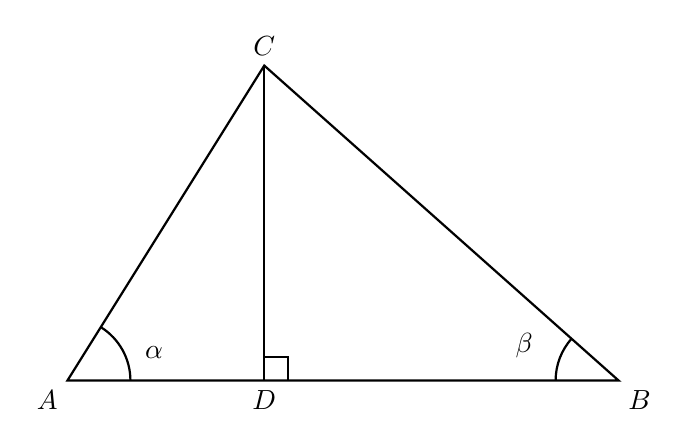
\begin{tikzpicture}
% Triangle vertices
\coordinate (A) at (0,0);
\coordinate (B) at (7,0);
\coordinate (D) at (2.5,0);
\coordinate (C) at (2.5,4);

% Triangle
\draw[thick] (A) -- (B) -- (C) -- cycle;

% Perpendicular line CD
\draw[thick] (C) -- (D);

% Right angle mark at D
\draw[thick] (D) ++(0.3,0) -- ++(0,0.3) -- ++(-0.3,0);

% Vertex labels
\node[below left] at (A) {$A$};
\node[below right] at (B) {$B$};
\node[above] at (C) {$C$};
\node[below] at (D) {$D$};

% Angle alpha at A
\draw[thick] (0.8,0) arc (0:58:0.8);
\node at (1.1,0.35) {$\alpha$};

% Angle beta at B
\draw[thick] (6.2,0) arc (180:138:0.8);
\node at (5.8,0.45) {$\beta$};
\end{tikzpicture}
\end{center}

Bereken hoek $\beta$ in graden en bereken de lengte van $BC$ en van $AB$.
